\documentclass[oneside, final, 14pt]{extreport}
\usepackage[utf8]{inputenc}
\usepackage[russianb]{babel}
\usepackage{vmargin}
\textwidth=16cm
\textheight=21cm
\oddsidemargin = 0pt
\setmarginsrb{2cm}{1.5cm}{1cm}{1.5cm}{0pt}{0mm}{0pt}{13mm}
\usepackage{indentfirst}
\usepackage{graphicx}
\usepackage{amsmath}
\usepackage{amssymb}
\usepackage{amsthm}
\sloppy

\newcommand\Chapter[1]{
	\refstepcounter{chapter}
	\chapter*{
		\begin{huge}
			\textbf{\arabic{chapter}.}
		\end{huge}%
		\bigskip \bigskip
		\raggedright #1
	}
	\addcontentsline{toc}{chapter}{\arabic{chapter}. #1}
}

\newcommand\Section[1]{
	\refstepcounter{section}
	\section*{\raggedright
		\arabic{chapter}.\arabic{section}. #1}
	\addcontentsline{toc}{section}{%
		\arabic{chapter}.\arabic{section}. #1}
}


\newtheorem{lem}{Лемма}
\newtheorem{thm}{Теорема}
\newtheorem{sled}{Следствие}
\newtheorem{alg}{Алгоритм}



\begin{document}
	%\fontsize{14}{16pt}\selectfont
	\renewcommand\contentsname{Содержание} %%% renaming the Table of Contents
	%\renewcommand\chaptername{}
	\thispagestyle{empty}
	
	\begin{center}
		\ \vspace{-1cm}
		
		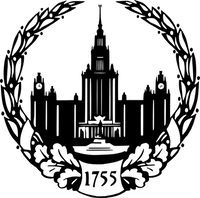
\includegraphics[width=0.2\textwidth]{logo-mgu.png}\\
		{\scshape Московский государственный университет имени М.~В.~Ломоносова}\\
		Факультет вычислительной математики и кибернетики\\
		Кафедра математической кибернетики
		
		\vfill
		
		{\LARGE Курсовая работа по теме}
		
		\vspace{1cm}
		
		{\Huge\bfseries <<Сложность расшифровки счетчика делимости на три>>}
	\end{center}
	
	\vspace{1cm}
	
	\begin{flushright}
		\large
		\textit{Студент 318 группы}\\
		М.\,М. Сакович
		
		\vspace{5mm}
		
		\textit{Научный руководитель}\\
		д.ф-м.н., доцент. С.\,Н. Селезнева
	\end{flushright}
	
	\vfill
	
	\begin{center}
		Москва, 2017
	\end{center}

	\tableofcontents
	\chapter*{Введение}
	\addcontentsline{toc}{chapter}{Введение}
	
	В работе рассматривается задача расшифровки функций из некоторого класса. Эта задача состоит в следующем. Нам нужно определить значения 
	на всех наборах некоторой функции $f$. При этом нам известно, что функция $f$ зависит от $n$ переменных и принадлежит некоторому классу
	функций $K$.
	Более того, мы можем задавать вопросы о значении функции $f$ на наборах и получать правильные ответы. Под сложностью расшифровки
	понимается число вопросов, которое следует задать, чтобы расшифровать любую функцию из класса $K$. Образно говоря, мы имеем дело 
	с "<черным ящиком">, у которого $n$ входов и один выход и про который известно, что он реализует некоторую функцию алгебры логики от $n$
	переменных из определенного класса $K$. Нам нужно определить, какую именно функцию он реализует.
	
	Рассмотрим множество $\{A\}$ алгоритмов, решающих поставленную задачу. Любой паре~--- алгоритму $A$ и функции $f(x_1, \ldots, x_n)$--- 
	можно сопоставить число $\varphi_K(A,f)$ вопросов о значении функции $f$ на наборах с помощью алгоритма $A$. Под сложностью  
	алгоритма $A$ понимаем функцию $\varphi_K(A,n) = \max\limits_{f \in K^n}\varphi_K(A, f)$, где $K^n$~--- множество всех функций от $n$ переменных
	из класса $K$. Под сложностью расшифровки класса $K$ понимаем функцию $\varphi_K(n) = \min\limits_A\varphi_K(A, n)$, где минимум берется по всем 
	алгоритмам $A$, решающим поставленную задачу.
	
	Впервые задача о расшифровке функций из некоторого класса была рассмотрена для монотонных функций. В 1963 году В. К. Коробков  \cite{korobkov}
	получил следующие оценки расшифровки класса монотонных функций $M$: 
	$$ \varphi_M(n) \geq C_n^{\lfloor \frac{n}{2} \rfloor} +  C_n^{\lfloor \frac{n}{2} \rfloor +1}.$$
	Окончательное решение этой задачи получил  Ж.Ансель в \cite{hansel}  
	$$ \varphi_M(n) = C_n^{\lfloor \frac{n}{2} \rfloor} +  C_n^{\lfloor \frac{n}{2} \rfloor +1}. $$

	В настоящее время важна задача расшифровки следующего вида. Пусть задана последовательность функций $g^k(x_1, \ldots, x_k)$,--- существенно 
	зависящих от $k$ переменных ($k = 0, 1, \ldots$), и рассмотрим класс $K$ функций, в котором $K^n$ содержит функции $g^k$, существенно зависящие  
	от переменных $x_{i_1}, \ldots, x_{i_k}$, $k = 0,1, \ldots, n$, $1 \leq i_1 < \ldots < i_k \leq n$. Поэтому, по сути, такая задача заключается в нахождении 
	существенных переменных функции $f$.
	
	В частности, в \cite{tokio} были рассмотрены классы: $K = OR$, где $g^k = x_1 \vee \ldots \vee x_k$; $K = PAR$, где $g^k = x_1 \oplus \ldots \oplus x_k$;
	$K = THR$, где $g^k$~--- это пороговая функция с пороговым значением $t$, $0 \leq t \leq k$. Из \cite{tokio} известно, что
	$$
	\begin{aligned}
		\varphi_{OR}(n) & = \varphi_{PAR}(n) = n \\
		\varphi_{THR}(n)&= n - 1 + \lceil \log_2(n+1) \rceil.
	\end{aligned} 
	$$
	
	Кроме того рассматриваются подзадачи расшифровки, когда число существенных переменных $k$ известно. В этом случае:
	$$
	\begin{aligned}
	       \lceil \log_2(С_n^k) \rceil & \leq \varphi_{OR(k)}(n) \leq k\lceil \log_2(\frac{n}{k}) \rceil + 2k - 2 \\
	        \lceil \log_2(С_n^k) \rceil & \leq \varphi_{PAR(k)}(n) \leq O(k\log_2(\frac{n}{k})) \\
	\lceil \log_2(kC_n^k + 2) \rceil & \leq \varphi_{THR(k)}(n) \leq 2(k-1)\log_2\left(\frac{n-1}{k-1}\right) + 6k - 6 + \lceil \log_2(n+2) \rceil.
	\end{aligned} 
	$$
	
	Отметим, что алгоритм $A$ расшифровки функций из класса $K$ можно представить в виде двоичного дерева, которое называется дерево решений
	\cite{kib}. Дерево решений $D_A$ ~--- это корневое ориентированное дерево, из любой вершины которого исходит не более двух дуг. Вершины, из 
	которых дуги не исходят, помечены функциями из $K^n$ и называются листьями, остальные вершины помечены наборами, которые задаются в вопросе.
	Если из вершины исходит две дуги, то они помечены $0$ и $1$ (условный переход) и если исходит одна дуга, то она без пометки (безусловный переход).
	Тогда сложностью $\varphi_K(A, n)$ ~--- это длина самой длинной цепи из корня в лист, не включая лист.  
	Из такого представления алгоритмов расшифровки сразу следует, что для любого класса $K$ 
	$$\varphi_K(n) \geq \lceil \log_2|K^n| \rceil,$$
	т.к. в дереве решений $D_A$ для каждой функции $f \in K^n$ должен быть лист, помеченный этой функцией. 
	
	В настоящей работе рассматривается  сложность задачи расшифровки счетчика делимости на $3$.
	
	\Chapter{Основные определения}
	Пусть $E_2 = \{0, 1\}$.
	Набор $(\alpha_1, \alpha_2, \ldots, \alpha_n)$, где $\alpha_i \in E_2, 1\leq i \leq n$, называется булевым или двоичным 
	набором (вектором). Элементы набора называют компонентами. Число $n$ называется длинной набора. Далее двоичный набор длины $n$ будем 
	обозначать $\tilde{\alpha}$.
	Множество всех двоичных наборов длины $n$ образует $n$-мерный булев (или двоичный) куб, который называют 
	также единичным $n$-мерным кубом и обычно обозначают $B^n$.
	 Весом  набора $\tilde{\alpha}$ (обозначение $ | \tilde{\alpha} | $) называют число его координат, равных $1$, т.е.  $$ | \tilde{\alpha} | = \sum_{i=1}^{n} \alpha_i.$$
	Наборы $\tilde{\alpha} \in B^n$ называют вершинами куба $B^n$. Множество всех вершин куба $B^n$, имеющих вес 
	$k$, называется $k$-м слоем куба  $B^n$ (обозначение $B_k^n$).
	Набор, все координаты которого равны $0$, будем называть нулевым. Набор, все координаты которого равны $1$ ~--- единичным. 
	Вес нулевого набора равен $0$, а вес единичного ~--- $n$.
	 Наборы будем называть соседними, если они различаются только в одной координате.
	 
	 Функция $f(x_1, \ldots, x_n)$, определенная на множестве $B^n = \{0,1\}^n$ и принимающая значения из множества 
	$\{0, 1\}$, называется функцией алгебры логики (булевой функцией). Множество всех булевых функций обозначим через $P_2$, множество 
	функций зависящих от $n$ переменных $x_1, \ldots, x_n$, через $P_2^n$.
	
	 Переменная $x_i \: (1 \! \leq \! i \!  \leq \! n)$ функции $f(x_1, \ldots, x_{i-1}, x_i, x_{i+1}, \ldots, x_n)$ называется существенной, 
	если можно указать такие наборы $\tilde{\alpha}$ и $\tilde{\beta}$, соседние по $i$-й компоненте, 
	(т.е $\tilde{\alpha} = (\alpha_1, \ldots, \alpha_{i-1}, 0, \alpha_{i+1}, \ldots, \alpha_n)$ и 
	$\tilde{\beta} = (\alpha_1, \ldots, \alpha_{i-1}, 1, \alpha_{i+1}, \ldots, \alpha_n)$), 
	что $f(\tilde{\alpha}) \not= f(\tilde{\beta})$.
	В противном случае переменная называется фиктивной. Если у функции все переменные фиктивные, то она является константой. 
	
	\Chapter{Постановка задачи}
	Рассмотрим функции: $\tau_0^ k(x_1, \ldots, x_k),  \tau_1^k(x_1, \ldots, x_k), \tau_2^k(x_1, \ldots, x_k) \in P_2^k$, такие что
	\[ \tau_i^k(\tilde{\alpha}) = \begin{cases}
		1, & |\tilde{\alpha}| \bmod 3 = i, \\
		0, & |\tilde{\alpha}| \bmod 3 \not = i.
	\end{cases}\]
	
    Пусть $A_i^n = \{\tau_i^k(x_{i_1}, \ldots, x_{i_k}) \mid 1 \leq i_1 < i_2 < \ldots < i_k \leq n, \, k=0,\ldots, n\} \,  i \in \{0, 1, 2\}.$

 \begin{figure}[h]
 	\begin{center}
 		\begin{minipage}[h]{0.3\linewidth}
 			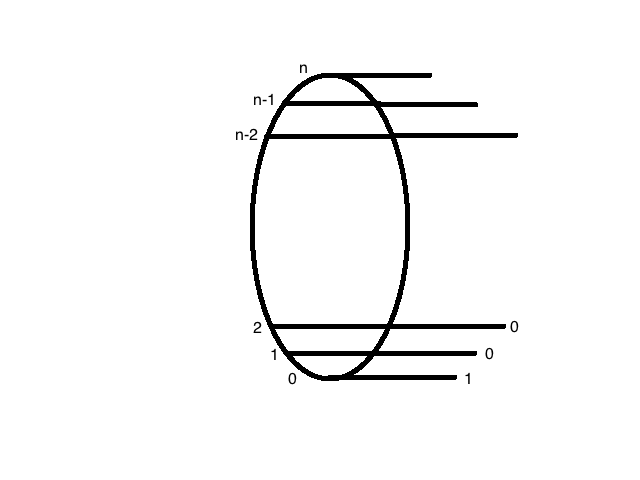
\includegraphics[width=1\linewidth]{A0}
 			\caption{Класс $A_0^n$.} %% подпись к рисунку
 			\label{ris:A0} %% метка рисунка для ссылки на него
 		\end{minipage}
 		\hfill 
 		\begin{minipage}[h]{0.3\linewidth}
 			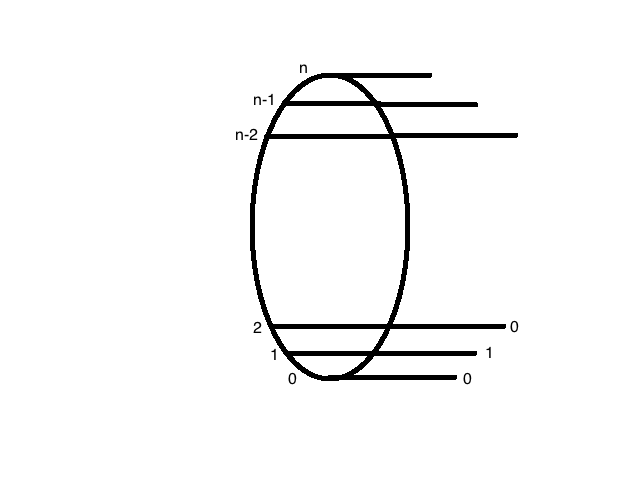
\includegraphics[width=1\linewidth]{A1}
 			\caption{Класс $A_1^n$.}
 			\label{ris:A1}
 		\end{minipage}
 		\hfill 
 		\begin{minipage}[h]{0.3\linewidth}
 		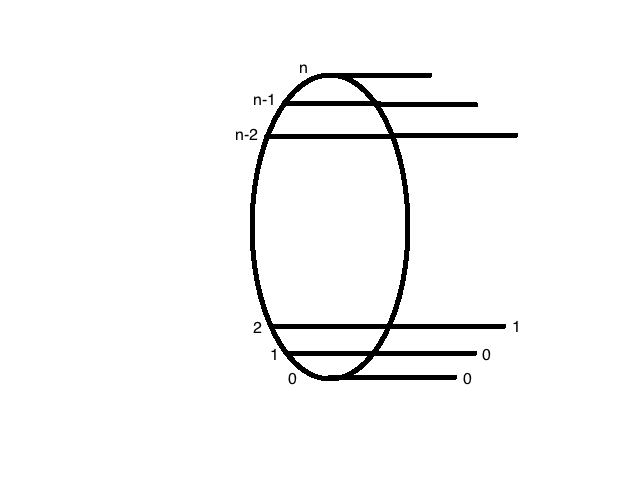
\includegraphics[width=1\linewidth]{A2}
 		\caption{Класс $A_2^n$.}
 		\label{ris:A2}
 	\end{minipage}
 	\end{center}
 \end{figure}

	Положим $A_i = \bigcup\limits_{n \geq 0}A_i^n$. Найдем сложность $\varphi_{A_i}(n)$ расшифровки функции из класса $A_i$, $i \in \{0,1,2\}$. 

	
	\Chapter{Основная часть}
	\Section{Решение} 
	\noindent Чтобы дать нижнюю оценку, посчитаем мощность классов $A_i^n \, (i = 0,1,2)$.
	\begin{lem}
		 \label{l1}
		 Для всех $n \geq 1$ справедливо $|A_0^n| = |A_1^n| = 2^n$. 
	\end{lem}
    \begin{proof}
		Рассмотрим класс $A_0^n$. Он порождается последовательностью функций $\tau_0^k(\tilde{x})$. Любая функция $f$ из этого класса зависит от
		$n$ переменных, среди которых любое число существенных. Из этих $n$ переменных 
		можем выбрать $0$ существенных переменных, т.е. $C_n^0$, $1$ существенную переменную, т.е. $C_n^1$ и т.д. 
		Таким образом, выбранный набор существенных переменных однозначно определяет функцию из класса.
	\[
		|A_0^n| = C_n^0 + C_n^1 + \cdots + C_n^n = \sum_{k=0}^{n}C_n^k = 2^n.
	 \]	
	
	\noindent Аналогично, $|A_1^n| = 2^n $. 
	\end{proof}
	\begin{lem}
	 \label{l2}
	 Для всех $n \geq 1$ справедливо $|A_2^n| = 2^n - n$.
	\end{lem}
	\begin{proof}
	 Класс $A_2^n$ порождается последовательностью функций $\tau_2^k(\tilde{x})$.Любая функция $f$ из этого класса зависит от $n$ переменных. 
	 В отличие от классов $A_0^n$ и $A_1^n$, если функция из класса $A_2^n$  существенно зависит от одной переменной, 
	 то она никогда не примет значение 1, значит мы не сможем распознать её. Таким образом 
	\[
		|A_2(n)| = C_n^0 + C_n^2 + \cdots + C_n^n = \sum_{k=0}^{n}C_n^k - C_n^1 = 2^n - n. 
	\]
	\end{proof}
	
	\begin{sled} 
	\label{s1}
	Для всех $n \geq 1$ справедливо
	\begin{displaymath}
		\begin{aligned}
			1.\, \varphi_{A_0}(n) \geq \lceil \log_2{|A_0(n)|} \rceil & = \log_2{2^n} = n  \\		
			2.\, \varphi_{A_1}(n) \geq \lceil \log_2{|A_1(n)|} \rceil & = \log_2[2^n] = n  \\
			3.\, \varphi_{A_2}(n) \geq \lceil \log_2{|A_2(n)|} \rceil & = \lceil \log_2(2^n - n) \rceil.  \\
		\end{aligned}
	\end{displaymath}
	\end{sled}
	
	\begin{lem}
		\label{log}
		При всех $ n > 2$ верно:
		$$\lceil \log_2(2^n - n) \rceil = n.$$
	\end{lem}
	\begin{proof}
		Из свойств логарифмов:
		\begin{displaymath}
		\begin{aligned}
		\lceil \log_2(2^n - n) \rceil & = \lceil \log_2(2^n) + \log_2(1 - \frac{n}{2^n}) \rceil =\\
												&= \lceil n + \log_2(1 - \frac{n}{2^n}) \rceil.	
	    \end{aligned}
		\end{displaymath}
		При $n > 2$ верно $\frac{n}{2^n} < 1$, последовательность $\frac{n}{2^n}$ убывает и ограничена нулем снизу. \\
		Значит  $ -1 < \log_2(1 - \frac{n}{2^n}) < 0$.
		Отсюда следует, что $\lceil \log_2(1 - \frac{n}{2^n})\rceil = 0 $, откуда $\lceil n + \log_2(1 - \frac{n}{2^n}) \rceil = n$.
	\end{proof} \par
	\bigskip
	\noindent Посмотрим, достигаются ли нижние оценки для классов $A_i^n \, (i= 0,1,2)$. \par
	\bigskip
	
	\noindent\textbf{Алгоритм $A_0$}. \\
	 \emph{\textbf{Вход:}} Функция $f \in A_0^n$.\\
	 \emph{\textbf{Выход:}} Существенные переменные функции $f \in A_0^n$.
	 \emph{Вопрос} $i$. Рассмотрим набор $\alpha_i = (0, 0,  \ldots, 0, 1, 0, \ldots, 0)$, в котором на $i$-м месте стоит $1$, а на всех остальных местах $0$.
	 Зададим $i$ для всех $i = 1, 2, \ldots, n$. Если $f(\alpha_i) = 0$, то переменная $x_i$ --- существенная. \\
	  
	 \begin{thm} 
	 	Алгоритм $A_0$ правильно расшифровывает класс $A_0$. 
	 \end{thm}
	 \begin{proof}
	 	Рассмотрим функцию $f$  из класса $A_0^n$ на нулевом наборе
	 	\[
	 	\tau_0(0, 0, \ldots, 0) =  \{0  \bmod 3 = 0\} = 1.
	 	\]
	 	Не задавая вопроса, мы знаем, что любая функция из класса $A_0^n$ на нулевом наборе имеет значение $1$.\\
	 	Если $f(\alpha_i) = 1$, то переменная $x_i$ не влияет на значение функции, т.е. $x_i$ --- 
	 	фиктивная переменная, в противном случае $x_i$ --- существенная \\
	 	Т.о. делаем $n$  запросов $\alpha_1, \alpha_2, \ldots, \alpha_n$ и для каждой из переменных $x_1, x_2, \ldots, x_n$ узнаем, является она существенной 
	 	или фиктивной. 
	 \end{proof} \par
	 
	\begin{thm} 
		При всех $n>0$ справедливо $\varphi_{A_0}(n) = n$.
	\end{thm}
	\begin{proof}
		Из следствия \ref{s1}: $\varphi_{A_0}(n) \geq n$. Алгоритм $A_0$ дает верхнюю оценку $\varphi_{A_0}(n) \leq n$. Следовательно 
		$\varphi_{A_0}(n) = n$.
	\end{proof} \par
	\noindent\textbf{Алгоритм $A_1$}. \\
	\emph{\textbf{Вход:}} Функция $f \in A_1^n$.
	\emph{\textbf{Выход:}} Существенные переменные функции $f \in A_1^n$.
	\emph{Вопрос} $i$. Рассмотрим набор $\alpha_i = (0, 0,  \ldots, 0, 1, 0, \ldots, 0)$, в котором на $i$-м месте стоит $1$, а на всех остальных местах $0$.
	Зададим вопрос $i$ для всех $i = 1, 2, \ldots, n$. Если $f(\alpha_i) = 1$, то переменная $x_i$ --- существенная. \\ 
	
	\begin{thm} 
		Алгоритм $A_1$ правильно расшифровывает класс $A_1$. 
	\end{thm}
	\begin{proof}
		Рассмотрим функцию $f$  из класса $A_1^n$ на нулевом наборе
		\[
		\tau_1(0, 0, \ldots, 0) =  \{0 \bmod  3 = 0\} = 0.
		\]
		Из этого следует, что не задавая вопроса, мы знаем, что любая функция из класса $A_1(n)$ на нулевом наборе имеет значение $0$.
		Заметим, что если функция $f$ существенно зависит от всех своих переменных, то на любом наборе из первого слоя, функция $f$ принимает
		значение $1$.\\
		Если $f(\alpha_i) = 0$, то переменная $x_i$ не влияет на значение функции, т.е. $x_i$ --- 
		фиктивная переменная, в противном случае $x_i$ --- существенная \\
		Т.о. делаем $n$  запросов $\alpha_1, \alpha_2, \ldots, \alpha_n$ и для каждой из переменных $x_1, x_2, \ldots, x_n$ узнаем, является она существенной 
		или фиктивной.
	\end{proof} \par
	
	\begin{thm} 
		При всех $n>0$  $\varphi_{A_1}(n) = n$.
	\end{thm}
	\begin{proof}
		Следствие \ref{s1} дает нижнюю оценку $\varphi_{A_1}(n) \geq n$. Алгоритм $A_1$ дает верхнюю оценку $\varphi_{A_1}(n) \leq n$. Следовательно 
		$\varphi_{A_1}(n) = n$.
	\end{proof}

	\noindent\textbf{Алгоритм $A_2$}. \\
	\emph{\textbf{Вход:}} Функция $f \in A_2^n$.\\
	\emph{\textbf{Выход:}} Существенные переменные функции $f \in A_2^n$.\\
	\emph{Шаг} 1. Рассмотрим набор $\tilde{\alpha_2} = (1, 1, 0, \ldots, 0)$. Если $f(\tilde{\alpha_2}) = 1$, то переходим к шагу 3. 
	В противном	случае переходим к шагу 2.\\
	\emph{Шаг} 2. Заменим в  наборе $\tilde{\alpha_i}$ первый встречающийся $0$ на  $1$, получим набор $\tilde{\alpha_{i+1}}$.
	Если $f(\tilde{\alpha_{i+1}}) = 1$, то переходим к шагу 3. Если набор
	 $\tilde{\alpha_{i+1}}$ --- единичный и $f(\tilde{\alpha_{i+1}}) = 0$, то все переменные функции $f$ --- фиктивные, иначе повторяем шаг 2.\\
	\emph{Шаг} 3. Последняя единица в наборе $\tilde{\alpha_k}$ стоит на $k$-м месте ($k \leq n$). Тогда переменная  $x_k$ - существенная.\\
	\emph{Шаг} 4. Построим набор 
	$${\alpha_{\lceil \frac{k-1}{2}\rceil_{k-1}}} = (1, 1, \ldots, 1, 0, \ldots, 0, 1, 0, \ldots, 0),$$
	 который получается из набора $\tilde{\alpha}$ заменой $1$, стоящих на местах $\lceil \frac{k-1}{2} \rceil, \lceil \frac{k-1}{2} \rceil + 1, \ldots, k-1$ на $0$. \\
	 Если $f({\alpha_{\lceil\frac{k-1}{2}\rceil_{k-1}}}) = 0$, то существенная переменная находится среди $x_{\lceil\frac{k-1}{2}\rceil}, \ldots, x_{k-1}$, в противном
	 случае существенная переменная среди $x_1, \ldots, x_{\lfloor \frac{k-1}{2} \rfloor}$. Таким образом мы сузили область поиска вдвое. 
	 Аналогичным образом 
	 будем заменять половину оставшихся $1$ на $0$, в зависимости  того, в какую половину попадает существенная переменная, до тех пор, пока не останется 
	 одна $1$, соответствующая переменной $x_i$. 
	 Переменная $x_i$ - является существенной. Пусть $\alpha_{ik} = (0, \ldots,0, 1, 0, \ldots, 0, 1, 0, \ldots, 0)$, где на $i$-м и  $k$-м местах стоят $1$, а на всех 
	 остальных $0$. Т.к. $x_i$ и $x_k$ - существенные, то  $f(\alpha_{ik}) = 1$. \\
	 \emph{Шаг} 5. Осталось найти все существенные переменные среди $n-k$ оставшихся. Для этого составим $n-k$ вопросов: 
	 
	 \begin{displaymath}
	 \begin{aligned}
	 	\alpha_{ik_1} & = (0, \ldots,0, 1, 0, \ldots, 0, 1, 1, 0, \ldots, 0) \\
	 	\alpha_{ik_2} & = (0, \ldots,0, 1, 0, \ldots, 0, 1, 0, 1, \ldots, 0) \\
	 	                    & \cdots \\
	 	\alpha_{ik_n} & = (0, \ldots,0, 1, 0, \ldots, 0, 1, 0, 0, \ldots, 1)
	 \end{aligned}
	 \end{displaymath}	
	 
	Если $f(\alpha_{ik_j}) = 1$ (где $j = k+1, \ldots, n$), то переменная $x_j$ - фиктивная. В противном случае $x_j$ - существенная.	
	\begin{thm} 
		Алгоритм $A_2$ правильно расшифровывает класс $A_2$. 
	\end{thm}
	\begin{proof}
		Среди переменных $x_1, x_2, \ldots, x_{k-1}$ ровно одна существенная, т.к. $\tau_2(\tilde{\alpha})$ может принять первый раз значение $1$ только в 
		том случае, если на месте двух первых встретившихся существенных переменных в наборе $\tilde{\alpha}$ стоят единицы, 
		а так как добавление единицы на $k$-е место обращает функцию $\tau_2(\tilde{\alpha})$ в $1$, то $x_k$ -  вторая существенная переменная, 
		а первая находится среди первых $k-1$ переменных. 	Посчитаем, сколько вопросов нам понадобилось. \\
		На первом шаге 1 вопрос. На втором шаге нам понадобилось $k-2$ вопроса, где $k \leq n$. На 5-м шаге  $n-k$. Четвертый шаг по сути является
		алгоритмом бинарного поиска, сложность которого $ \leq \log_2(n)$. Таким образом, в худшем случае сложность приведенного алгоритма равна 
		$1 + k - 2 + n - k + \log_2(n) = n - 1 + log_2(n)$. 
	\end{proof} 	
	\begin{thm} 
		При всех $n > 0$ $\varphi_{A_2}(n) \sim n$.
	\end{thm}
	\begin{proof}
		Из Л.~\ref{log} и С.~\ref{s1}: при $n > 2$ $\varphi_{A_2}(n) \geq n$. Рассмотрим случаи, когда $n=1$ и $n=2$. \\
	    При $n = 1$ функция $f(|\alpha|) \in A_2(n)$ является константой, так как никогда не примет значение $1$. При $n=2$ $\varphi_{A_2}(2) \geq 1$. 
	    Получим верхнюю оценку. Зададим вопрос $\alpha(1, 1).$ Если $f(\alpha) = 1$, то обе переменные существенные, в противном случае функция является
	    константой. Таким образом для $n = 1,2$  $\varphi_{A_2}(n) = n-1$.\\
	    При $n > 2$ алгоритм $A_2$ дает верхнюю ассимптотическую  оценку $\varphi_{A_2}(n) \lesssim n$. Следовательно $\varphi_{A_2}(n) \sim n$.
	\end{proof}	

	\Section{Результаты}
	
	В работе получены следующие результаты: 
	
	$\varphi_{A_0}(n) = \varphi_{A_1}(n) = n,$
	
	$\varphi_{A_2}(n) \sim n$ при $n \rightarrow \infty.$
	
	\begin{thebibliography} {0}
		\addcontentsline{toc}{chapter}{Литература}
		
		\bibitem{korobkov} Коробков В.К. \emph{О монотонных функциях алгебры логики.} Сб. Проблемы кибернетики. Вып 13. М.: Наука, 1965. --- С.~5--27.
		
		\bibitem{hansel} Ансель Ж. \emph{О числе монотонных булевых функций от $n$ переменных.} В кн. Кибернетический сборник. Новая серия. Вып. 5. 
		М.: Мир, 1968. --- С.~53--57.
		
		\bibitem{tokio} Ryuhei Uehara, Kensei Tsuchida, Ingo Wegener \emph{Optimal attribute-efficient learning of disjunction, parity, and threshold functions}. 1996.
		
		\bibitem{kib} Ахо А., Хопкрофт Дж., Ульман Дж. \emph{Построение и анализ вычислительных алгоритмов.} М.: Мир, 1979.
		
		\bibitem{gavrilov:sapogenko} Гаврилов Г.П., Сапоженко А.А. \emph{Сборник задач по дискретной математике.} М.: ФИЗМАТЛИТ, 2004.
		
		\bibitem{alekseev} Алексеев В.Б. \emph{Введение в теорию сложности алгоритмов.} М.: Изд. отдел ф-та ВМиК МГУ, 2002.
		
	\end{thebibliography}
\end{document}
